\documentclass{article}
\usepackage[utf8]{inputenc}

%% Sets page size and margins
\usepackage[a4paper,top=3cm,bottom=2cm,left=3cm,right=3cm,marginparwidth=1.75cm]{geometry}
\usepackage{setspace}
%% Useful packages
\usepackage{listings}
\usepackage{caption}
\usepackage{amssymb,amsmath,amsthm}
\usepackage{mathtools} \usepackage{graphicx}
\usepackage[colorlinks=true, allcolors=blue]{hyperref}
\usepackage{float}
\usepackage{enumerate}
\usepackage{subcaption}
\usepackage{hyperref}
\usepackage[table,xcdraw]{xcolor}
\usepackage{tikz}

\newcommand{\Lagr}{\mathcal{L}}
\newcommand\norm[1]{\left\lVert#1\right\rVert}
\DeclareMathOperator*{\argmin}{arg\,min} 
\usepackage{tikz-cd}
\usepackage{rotating}
\newtheorem{theorem}{Teorema}
\newtheorem{definition}{Definición}
\newtheorem*{proposition}{Proposición}
\newtheorem*{corollary}{Corolario}
\newtheorem*{example}{Ejemplo}
\newtheorem*{lemma}{Lema}
\newtheorem{observation}{Observación}

\usepackage{fancyhdr}
\pagestyle{fancy}
\thispagestyle{empty}
\onehalfspacing

\begin{document}

\title{Recurrent harmonizer}

\author{José Pablo Ortiz}
\maketitle
\section*{Introduction}
In this work a deep learning model, many-to-many recurrent neural network, will be developed to harmonize a melody in the style of Bach. For this end, the Bach 2/3 part inventions are gonna be used as the data to train the model; it's the first time a recurrent music generation model has been used to fit this data. Most of the previous work that has been used to model Bach's music use the chorales.
\noindent
In the first part we are gonna introduce the context and characteristic of the inventions along with the pianoroll notation. Then, in the second part a short yet concise exposition of the model will be outlined. In the final part, the details of the training, the model selection and the results will be shown.


\section*{Data}
The inventions by Johann Sebastian Bach are a 30 piece collection for the keyboard. They are composed as 2 or 3 voice polyphonic pieces. A 2/3 voice polyphonic piece is consists of 2/3 independent melodies, with the property that when played together they sound harmonious. Figure 1 shows the sheet music of one measure of a 2 voice invention. The upper bunch of notes represent the first melody and the lower the second one.
\noindent
The sheet music of all the inventions was obtained from Musescore and then hand preprocessed in order to make the data extraction process more uniform. The information was extracted using the python library \textsc{music21}. \textsc{music21} is an amazing python library with a series of tools 'for helping scholars and other active listeners answer questions about music quickly and simply'
\begin{figure}[H]
\begin{minipage}{.4\textwidth}
  \centering
  \includegraphics[width=.6\linewidth]{Images/polyphonic.png}
  \captionof{figure}{A two part invention}
  \label{fig:test1}
\end{minipage}%
\begin{minipage}{.5\textwidth}
  \centering
  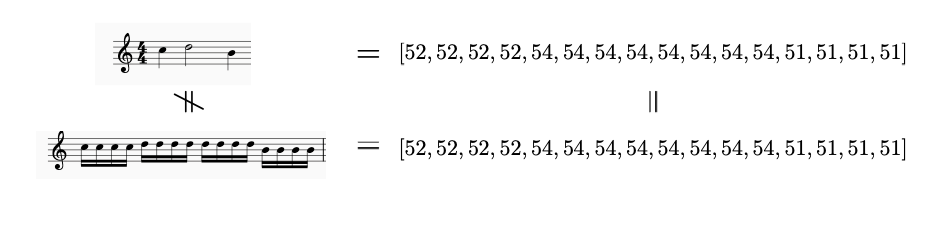
\includegraphics[width=1.3\linewidth]{Images/PianoRollProblem.png}
  \captionof{figure}{An example on how the piano roll misses some information about a melody. }
  \label{fig:test2}
\end{minipage}
\end{figure}


\subsection*{Piano Roll}

The data format that it is used in this project is the piano roll notation. In the context of music generation using deep learning it was first used by Boulanger-Lewandowski\cite{Boulanger-Lewandowski}. To represent a sheet music of a 1 voice melody as a piano roll, first it is need to establish the smallest time duration of every note or rest in the sheet music. Then every piece can be seen as  finite time discrete sequence of notes; where every time instant has the duration of the smallest note duration. Representing every note as one of the 88 keys in a keyboard and a rest by the number $-1$. This yields, that a 1 voice melody piece can be seen as sequence $\{v_{t}\}_{t=1}^D$ where $v_t$ is the number of note played at time $t$. 
\noindent
The piano roll notation misses some information about the music. Let's suppose that the smallest note duration of a one voice melody is $\frac{1}{16}$ and that there exists a $k$ and $n$ such that $v_{k}=v_{k+1}=\dots = v_{k+n}$; then the piano roll notation will not be able to gather information of whether the note $v_{k}$ is played $n$ times or has duration $\frac{n}{16}$. An example of this it is shown in Figure 2. 
\begin{figure}[H]
\includegraphics[width=10cm]{Images/duration.png}
\centering
\caption{Diagram explaining the duration of notes.}
\end{figure}
\noindent
For the dataset in this work we will only take inventions in which the smallest note duration is $\frac{1}{16}$. A two voice invention following the piano roll notation can be written as
$$I = \left\{(v^{1}_t,v^{2}_t)\right\}_{t=1}^D$$
where $v^{i}_t$ represent the note a time $t$ of the $i$-th voice and $D$ the duration of the invention. Thus, each time $t$ represents $\frac{1}{16}$ note and the duration of the invention is $\frac{D}{16}$.
In the other hand, a three voice invention can be written as
$$I = \left\{(v^{1}_t,v^{2}_t,v^{3}_t)\right\}_{t=1}^D.$$
Nonetheless, this work will focus on adding a another voice to a melody. So, in order to use the data of the 3 voice inventions we will extract two 2 voice inventions for every 3 voice invention in the following way:
$$I_1 = \left\{(v^{1}_t,v^{2}_t)\right\}_{t=1}^D\quad I_2 = \left\{(v^{2}_t,v^{3}_t)\right\}_{t=1}^D.$$ 


\subsection*{Data Augmentation}
We can do data augmentation by adding some constant to every note. Because there are 12 tones, in order to not be redundant in a musical way, it is only possoble to add 12 consecutive integers $\{-6,-5,\dots,6\}$. Thus, by doing this data augmentation the dataset has 11 more observations per observation.
\begin{table}[H]
\begin{tabular}{|l|l|l|}
\hline
2 voice Invention & Number of different notes & Number of different notes with data augmentation \\ \hline
voice 1 & 34 & 45 \\ \hline
voice 2 & 39 & 50 \\ \hline
\end{tabular}
\caption{}
\end{table}


\begin{table}[H]
\begin{tabular}{|l|l|l|}
\hline
3 voice Invention & Number of different notes & Number of different notes with data augmentation \\ \hline
voice 1 & 27 & 39 \\ \hline
voice 2 & 33 & 45 \\ \hline
voice 3 & 39 & 50 \\ \hline
\end{tabular}
\caption{}
\end{table}

\begin{table}[H]
\begin{tabular}{|l|l|l|}
\hline
2 and 3 voice Invention & Number of different notes & Number of different notes with data augmentation \\ \hline
voice 1 & 37 & 48 \\ \hline
voice 2 & 47 & 59 \\ \hline
\end{tabular}
\caption{}
\end{table}

\subsection*{One Hot Encoding}
The one hot encoding consists in assigning every note used in an invention a canonical vector of dimension the size of notes used in an invention. Given Table 3 every note in voice 1 will be represented as a canonical vector of dimension 48 and voice 2 as a canonical vector of dimension 59. From now on, the sequence $\{v_t\}_{t=1}^D$ will be the one hot encoding of a melody; that is, a sequence of canonical vectors.  
\noindent
Another advantage of using the one hot encoding is that we can visualize a whole piece as shown in Figure 4 where a one hot encoding was taken with a number of notes of 88.

\begin{figure}[H]
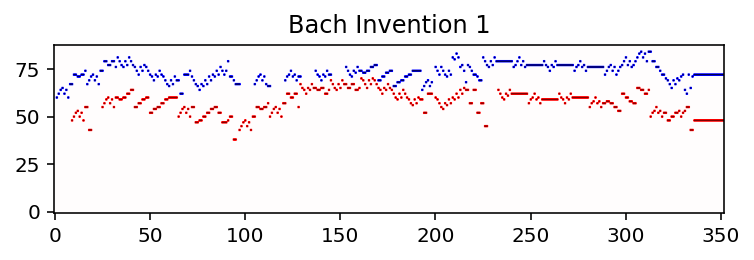
\includegraphics[width=10cm]{Images/BachPianoRoll.png}
\centering
\caption{Visualization of Bach's invention no. 1}
\end{figure}


\subsection*{Rolling Window}

The model that is gonna be trained is a many-to-many deep recurrent neural network of size $T$. In order to train the model it is necessary to obtain all the rolling windows of size $T$ and stride $s$ of the inventions. The rolling windows of size $T$ and stride $s$ of an invention are
\begin{equation*}
\left\{\left[(v^{1}_{ks+t},v^{2}_{ks+t})\right]_{t=1}^{T}|\quad\text{ for } k=0,1,\dots,\frac{D-T}{s}\right\}.
\end{equation*}
\noindent
The aim of this project is to create a model that given a melody of high notes it adds a second melody of bass notes so that when played together they sound harmonious. For this end, it's necessary to have information about the current melody of voice and the bass melody. So the input of the model will have the form
\begin{equation}
X=\begin{pmatrix}
X_{11}&X_{12}&\dots,X_{1T}\\
X_{21}&X_{22}&\dots,X_{2T}\\
\end{pmatrix} = \begin{pmatrix}
v^{1}_{ks}&v^{1}_{ks+1}&\dots& v^{1}_{ks+T}\\
v^{2}_{ks-1}&v^{2}_{ks}&\dots& v^{1}_{ks+T-1}\\
\end{pmatrix},
\end{equation}
and the output
\begin{equation}
Y =\begin{pmatrix}
Y_{1}&Y_2&\dots,Y_T\\
\end{pmatrix} =  \begin{pmatrix}
v^{2}_{ks}&v^{2}_{k+1}&\dots& v^{2}_{ks+T}
\end{pmatrix}.
\end{equation}

\section*{Recurrent Harmonizer}


\begin{figure}[H]
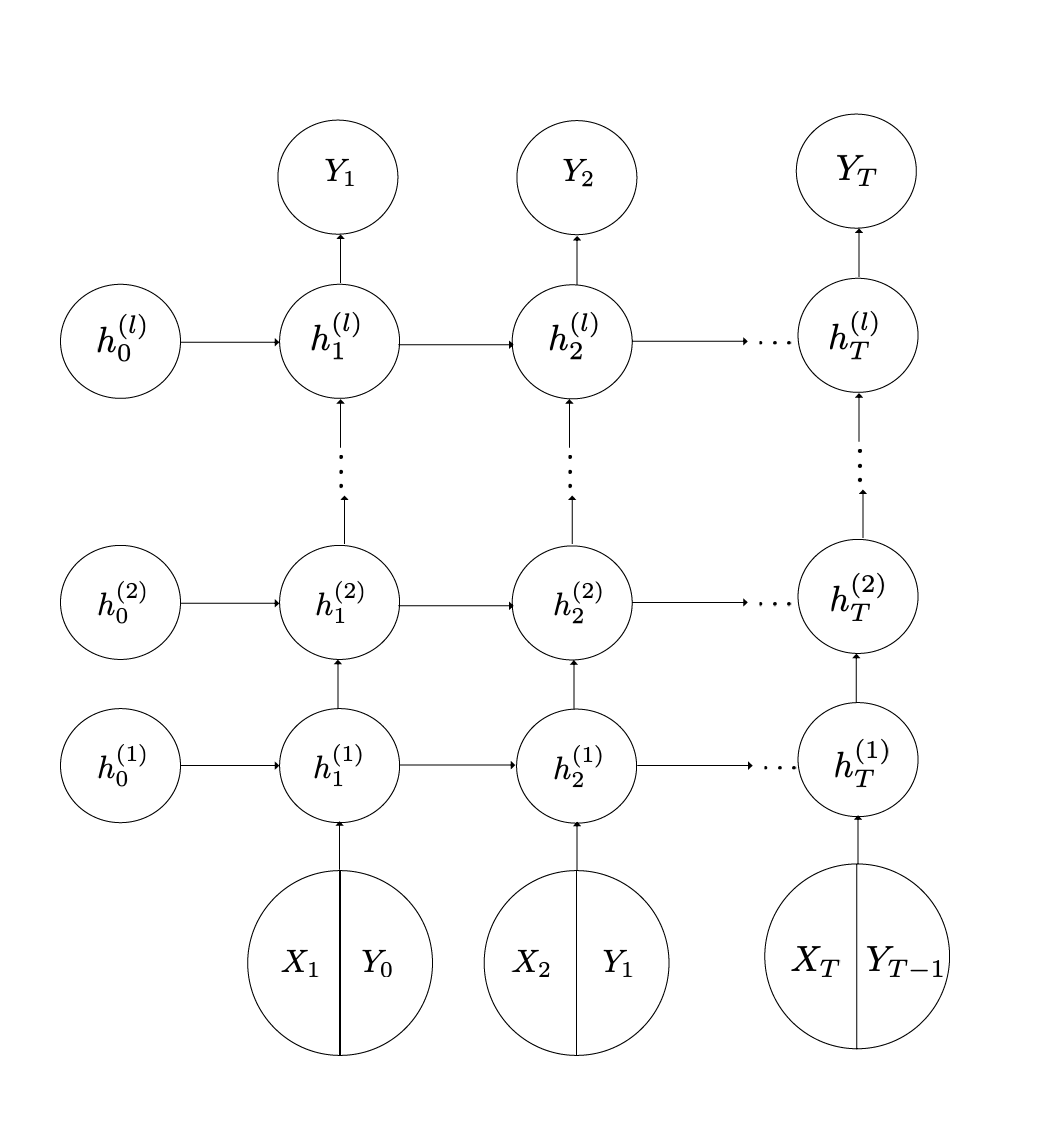
\includegraphics[width=8cm]{Images/ManyToManyRnn.png}
\centering
\caption{Diagram explaining the duration of notes.}
\end{figure}

\subsection*{Model}
The many-to-many RNN is probabilistic generating model, it is a generative because the task is to predict the conditional probability mass function
\begin{equation}
p(y_t|y_{t-1},\dots,y_0,x_t,\dots,x_1).
\end{equation}
As mentioned earlier a many-to-many deep RNN of size $T$ consists of the following discrete time recurrence equations
\begin{equation}
	\begin{split}
		h^{(1)}_t &= g\left(W^{(1)}h_{t-1}+U^{(1)}_1(X_{1t})+U^{(1)}_2(X_{2t})\right)\\
		h^{(2)}_t &= g\left(W^{(2)}h^{(1)}_{t}+U^{(2)}h^{(2)}_{t-1}\right)\\
		\vdots\\
		h^{(l)}_t &= g\left(W^{(l)}h^{(l-1)}_{t}+U^{(l)}h^{(l-1)}_{t-1}\right) \\
		\hat{p}(y_t|y_{t-1},\dots,y_0,x_t,\dots,x_1)=\hat{p}(y_t|h^{(1)}_t,\dots,h^{(l)}_t)&= \mbox{softmax}(Vh^{(l)}_t),
	\end{split}
\end{equation}
 for $t=1,\dots,T$. By abusing notation $g$ represents a Long Short Term Memory cell, $X$ and $Y$ are the input and output as in (1) and (2), $l$ the depth of the neural network, and $h^{(\cdot)}_t$ the hidden states. The entries of the matrices $W^{(\cdot)},U^{(\cdot)}$ and $V$ are the weights/coefficients that are up to estimation. The dimension of this matrices are known as the number of neurons in a layer and they are hyperparameters of the model. Because we want to predict a probability, the function $\mbox{softmax}$ it's used as the last activation of the RNN. 
The idea behind this model is that the hidden space $h^{(i)}_t$ has the information about the process up until time $t$; in a more mathematical way, that is $h^{(i)}_t\subset \sigma (Y_0,\dots,Y_{t-1},X_1,\dots,X_t)$ where $ \sigma (Y_0,\dots,Y_{t-1},X_1,\dots,X_t)$ is the sigma algebra generated by the random variables $(Y_0,\dots,Y_{t-1},X_1,\dots,X_t)$\cite{Calin}.
\subsection*{Inference or second voice generation}
Once the model is trained and given a melody $X=[X_1,\dots,X_T]$ and an initial value $Z_0$ it is possible to do inference(or creating a second voice) by following the recursion
\begin{equation}
	\begin{split}
		Z_1 &= \arg\max \{p(Z_1|Z_0,x_1)\}\\
		Z_2 &= \arg\max \{p(Z_2|Z_1,Z_0,X_1,X_2)\}\\
		\vdots&\\
		Z_T &=  \arg\max \{p(Z_t||Z_{T-1},\dots,Z_{0},X_1,\dots,X_T))\}
	\end{split}
\end{equation}



\subsection*{Hyperparameters of the model}
$l$ represents the depth or number of layers in a neural network. Let $c_1$ and $c_2$ be the number of notes in voice 1 and 2, then the matrices $U^{(1)}_1\in\mathbb{R}^{c_1\times n_1}$ and $U^{(1)}_2\in\mathbb{R}^{c_2\times n_1}$ where $n_{1}$ is the numbers of neurons in the first layer. For $i=2,\dots l$ we have that $U^{(i)}\in\mathbb{R}^{n_{i-1}\times n_i}$; meanwhile $W^{(i)}\in\mathbb{R}^{n_i\times n_i}$. The hyperparameter $n_i$ represents the number of neurons in the $i$-th layer. The trade off of this hyperparameters is that more depth and more neurones per layer can offer more flexibility but can overfit the data and make it harder to train the model. 



\section*{Training and model selection}

To train the model first we need set the size and the stride of the rolling window as in (1) to generate the training data $X$ and $Y$. We will set $T = 32$ and $s=1$ to generate the training data to obtain a sample of $52284$ rolling windows. This $52284$ were split in an $n = (80\%)$ training set and $n_{\mbox{val}} = (20\%)$ validation set. We acknowledge that the model selection
\subsection*{Loss function and numerical minimization}
Because we want to make inference on a probability function the loss function that is gonna be used is the cross entropy; that is:
\begin{equation}
\frac{1}{n} \sum_{i=1}^nL_i =\frac{1}{n} \sum_{i=1}^n \left[\frac{1}{T}\sum_{t= 1}^T\log\left(\hat{p}(y_t|h^{(1)}_t,\dots,h^{(l)}_t))\right)\right],
\end{equation}
where $L_i$ is the loss of each observation. Thus, in order to estimate the weight matrices we need to minimize (7). The algorithm that it's used to minimize(6) is minibatch stochastic gradient descent with the gradient, calculated by backpropagation, being updated using the ADAM method.

Table 4 shows the different metrics to judge the performance of our different models. For our final model we are gonna select the one with the validation accuracy closest to 1. That is the one with $l=2$ and each layer with 512 neurons. 

 
\begin{table}[h]
\begin{tabular}{|
>{\columncolor[HTML]{FFFFFF}}c |
>{\columncolor[HTML]{FFFFFF}}c |
>{\columncolor[HTML]{FFFFFF}}c |
>{\columncolor[HTML]{FFFFFF}}c |
>{\columncolor[HTML]{FFFFFF}}c |c|}
\hline
{\color[HTML]{212121} \textbf{layers}} & {\color[HTML]{212121} \textbf{hidden}} & {\color[HTML]{212121} \textbf{train loss}} & {\color[HTML]{212121} \textbf{train accuaricy}} & {\color[HTML]{212121} \textbf{val\_loss}} & {\color[HTML]{212121} \textbf{val\_sparse\_categorical\_accuracy}} \\ \hline
{\color[HTML]{212121} 1} & {\color[HTML]{212121} 32} & {\color[HTML]{212121} 1.40} & {\color[HTML]{212121} 0.59} & {\color[HTML]{212121} 1.40} & {\color[HTML]{212121} 0.59} \\ \hline
{\color[HTML]{212121} 1} & {\color[HTML]{212121} 64} & {\color[HTML]{212121} 1.22} & {\color[HTML]{212121} 0.64} & {\color[HTML]{212121} 1.23} & {\color[HTML]{212121} 0.64} \\ \hline
{\color[HTML]{212121} 1} & {\color[HTML]{212121} 128} & {\color[HTML]{212121} 0.91} & {\color[HTML]{212121} 0.73} & {\color[HTML]{212121} 0.92} & {\color[HTML]{212121} 0.72} \\ \hline
{\color[HTML]{212121} 1} & {\color[HTML]{212121} 256} & {\color[HTML]{212121} 0.44} & {\color[HTML]{212121} 0.88} & {\color[HTML]{212121} 0.47} & {\color[HTML]{212121} 0.87} \\ \hline
{\color[HTML]{212121} 1} & {\color[HTML]{212121} 512} & {\color[HTML]{212121} 0.20} & {\color[HTML]{212121} 0.94} & {\color[HTML]{212121} 0.25} & {\color[HTML]{212121} 0.93} \\ \hline
{\color[HTML]{212121} 2} & {\color[HTML]{212121} 64,64} & {\color[HTML]{212121} 1.11} & {\color[HTML]{212121} 0.67} & {\color[HTML]{212121} 1.12} & {\color[HTML]{212121} 0.67} \\ \hline
{\color[HTML]{212121} 2} & {\color[HTML]{212121} 128,128} & {\color[HTML]{212121} 0.62} & {\color[HTML]{212121} 0.83} & {\color[HTML]{212121} 0.64} & {\color[HTML]{212121} 0.82} \\ \hline
\cellcolor[HTML]{FFCCC9}{\color[HTML]{212121} 2} & \cellcolor[HTML]{FFCCC9}{\color[HTML]{212121} 256,256} & \cellcolor[HTML]{FFCCC9}{\color[HTML]{212121} 0.25} & \cellcolor[HTML]{FFCCC9}{\color[HTML]{212121} 0.93} & \cellcolor[HTML]{FFCCC9}{\color[HTML]{212121} 0.29} & \cellcolor[HTML]{FFCCC9}{\color[HTML]{212121} 0.92} \\ \hline
{\color[HTML]{212121} 3} & {\color[HTML]{212121} 64,32,64} & {\color[HTML]{212121} 1.23} & {\color[HTML]{212121} 0.64} & {\color[HTML]{212121} 1.23} & {\color[HTML]{212121} 0.64} \\ \hline
{\color[HTML]{212121} 3} & {\color[HTML]{212121} 128,64,128} & {\color[HTML]{212121} 0.74} & {\color[HTML]{212121} 0.79} & {\color[HTML]{212121} 0.76} & {\color[HTML]{212121} 0.78} \\ \hline
{\color[HTML]{212121} 3} & {\color[HTML]{212121} 256,128,256} & {\color[HTML]{212121} 0.29} & {\color[HTML]{212121} 0.92} & {\color[HTML]{212121} 0.33} & {\color[HTML]{212121} 0.91} \\ \hline
\end{tabular}
\caption{The metrics of all the trained models}
\end{table}

\noindent

\subsection*{Results}
In order to show the results of the model we will use the prelude from Bach cello suite no 1. The piano roll of the result is shown in Figure 6

Hearing the results, it seems that the model has success in creating a Bach sound. Nonetheless, it's not able to capture the information about the long term structure of the piece.

\begin{sidewaysfigure}
    \centering
	\begin{figure}[H]
	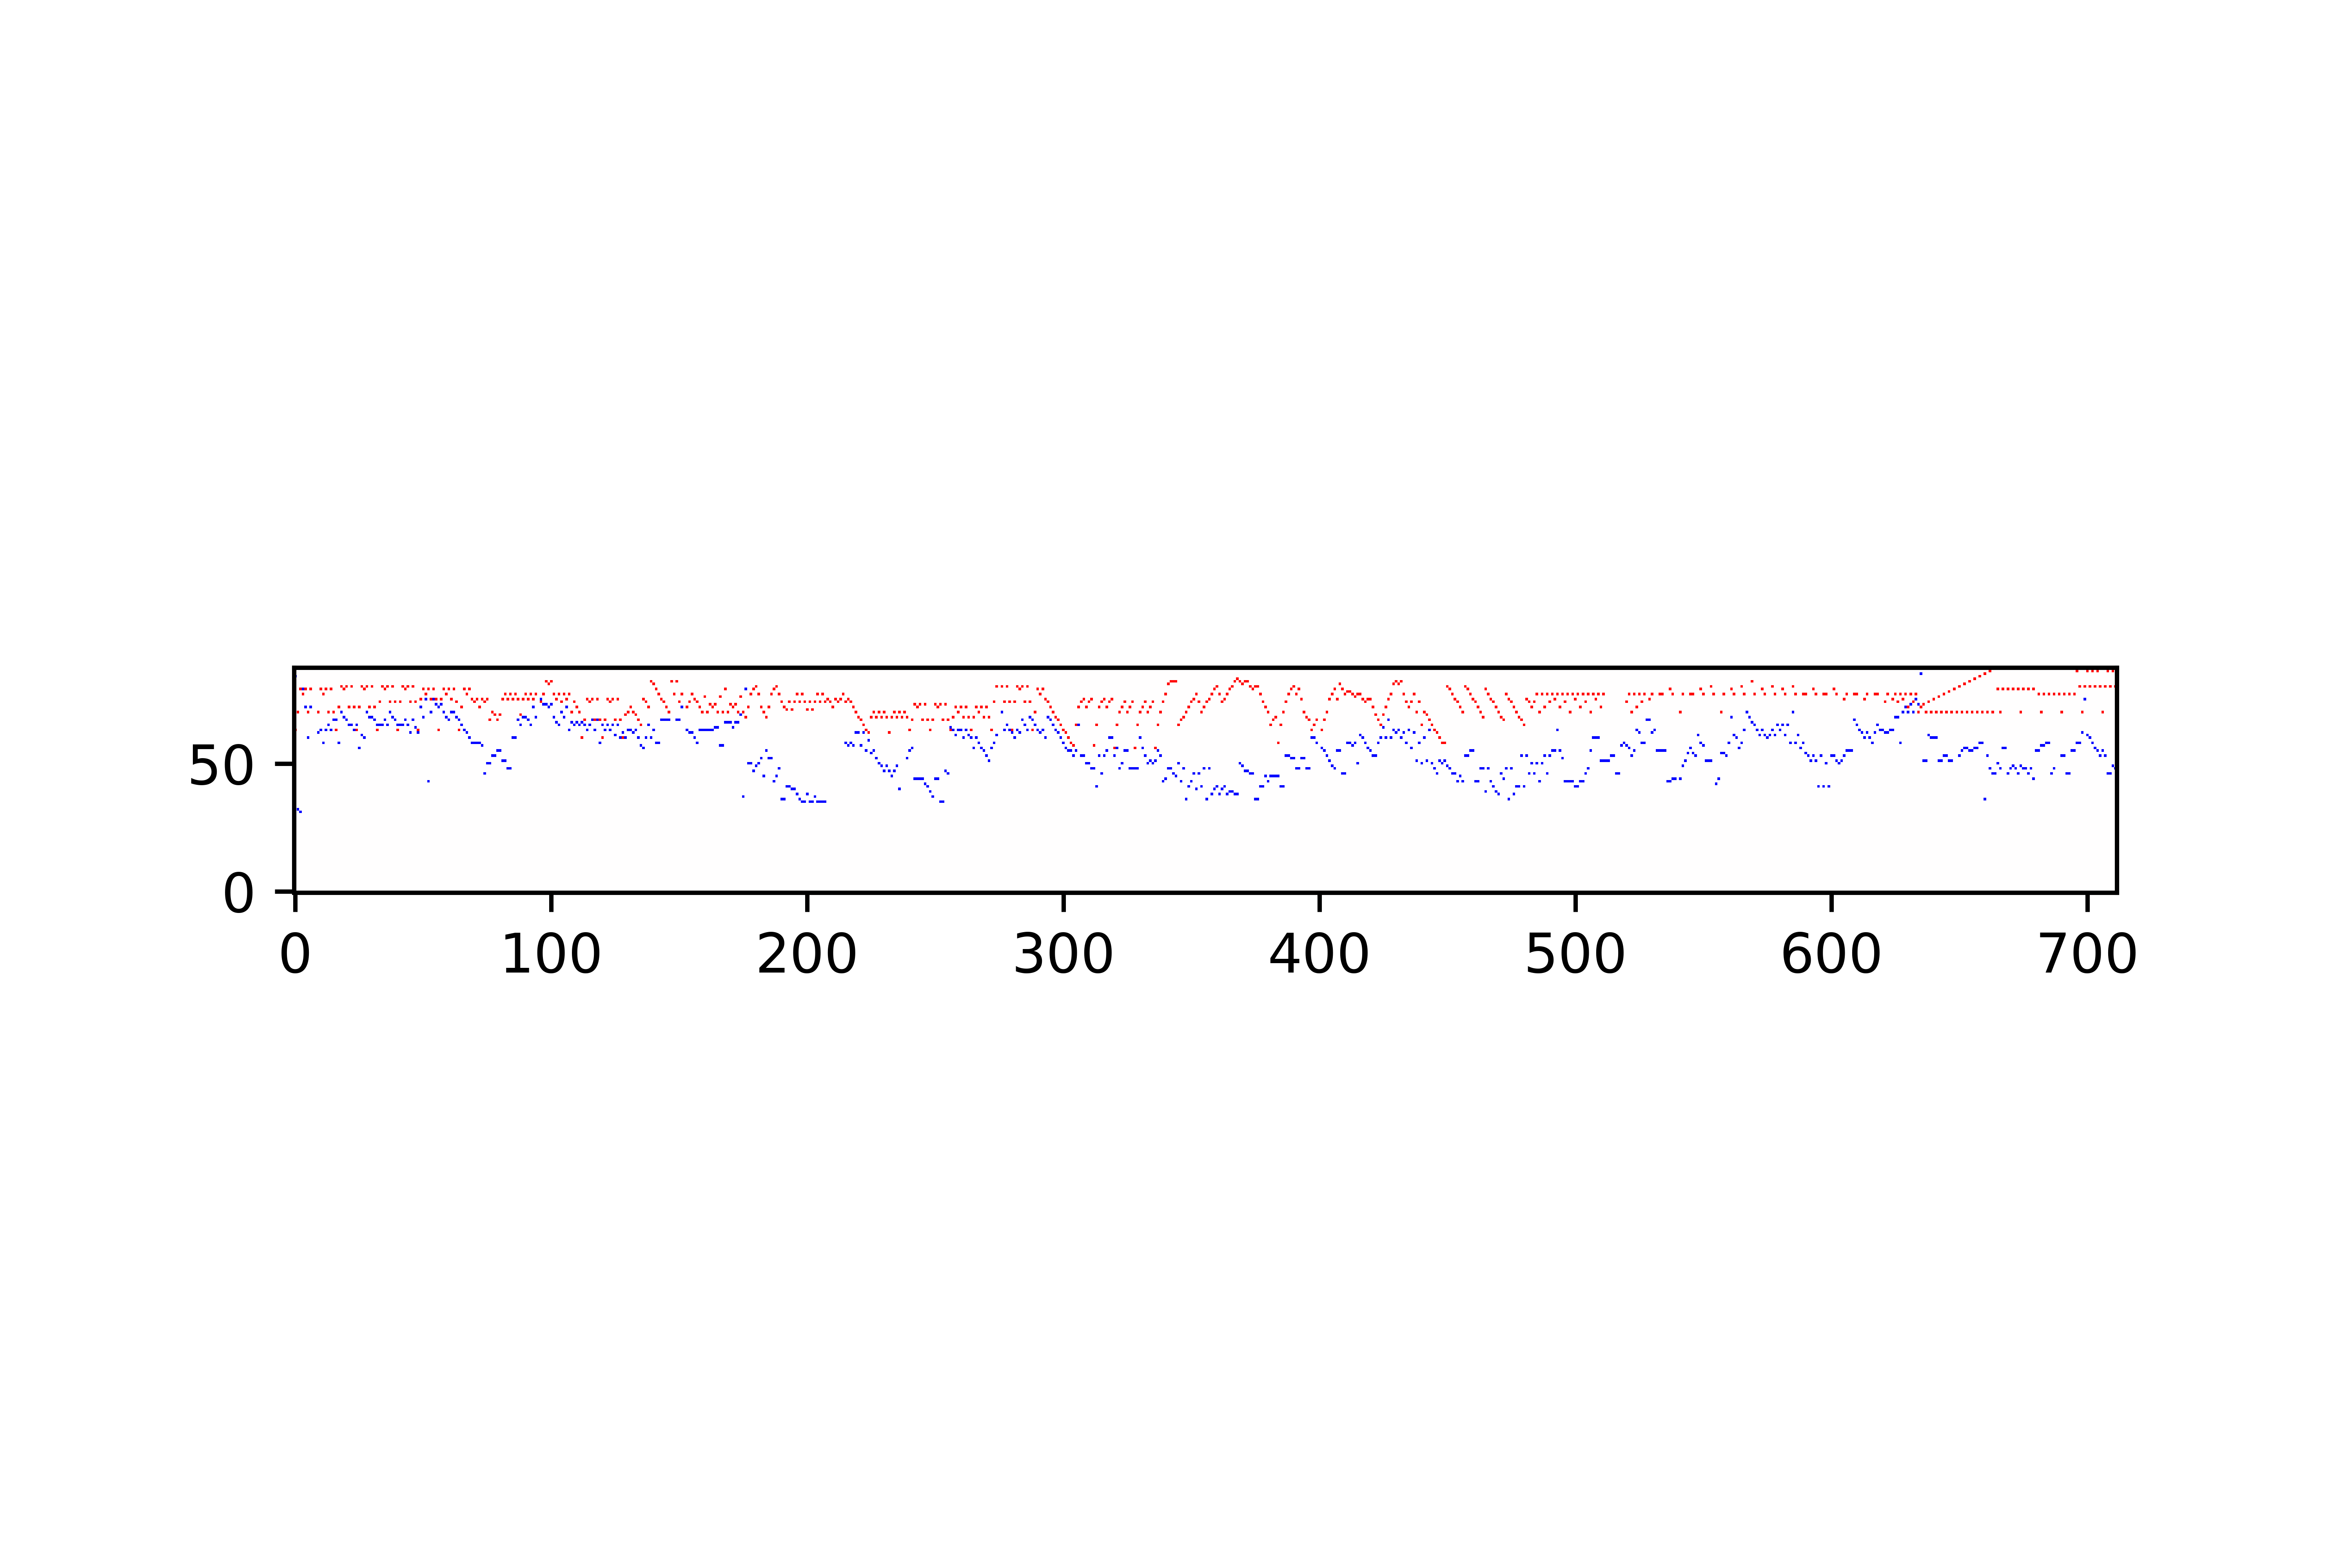
\includegraphics[width=30cm]{Images/PreludeHarmony.png}
	\caption{Diagram explaining the duration of notes.}
	\end{figure}
    \label{fig:awesome_image}
\end{sidewaysfigure}
\begin{thebibliography}{9}

\bibitem{Boulanger-Lewandowski}
Boulanger-Lewandowski, N., Bengio, Y.,\& Vincent, P.(2012). \textit{Modeling Temporal Dependencies in High-Dimensional Sequences: Application to Polyphonic Music Generation and Transcription}. ICML 2012: Edinburgh, Scotland.

\bibitem{Calin}
Calin, O. (2020). \textit{Deep Learning Architectures: A Mathematical Approach}  (1st ed.). Springer.
\end{thebibliography}

\end{document}










